%
%
\documentclass{article}
\usepackage{amsmath}
\usepackage{graphicx}
\usepackage{color}
\usepackage{caption}
\usepackage{amsfonts}
%\usepackage[margin=3cm]{geometry}
\usepackage{tikz}
\newcommand{\bs}{\boldsymbol}                               %

\begin{document}

\title{Numerical methods}
\author{Dominic Skinner}
\maketitle

Consider the govering equations
\begin{equation}\label{eq1}
\left( \begin{array}{c} p(z) \\ 0 \end{array} \right) =
 \left( \begin{array}{c} \sigma_y \\ \tau_{xy} \end{array} \right) =
\int_0^{\infty} \left(
\begin{array}{cc} K_{11}(x-z) & K_{12}(x-z) \\ K_{21}(x-z) & K_{22}(x-z) 
\end{array} \right)
 \left( \begin{array}{c} g'(x) \\ h'(x) \end{array} \right) dx
\end{equation}
%
\begin{equation}\label{eq2}
h^2p'=\lambda
\end{equation}
Have the ``input'' parameters as 
\begin{itemize}
\item BC's $P$, $M$ (or equivalently $g'$, $h''$ at $x\to\infty$)
\item $\lambda$ , the speed
\end{itemize}
Want to solve for the toughness $K_I$ and $K_{II}$. In this project,
we have so far focused on $K_I$.
\begin{figure}[!ht]\centering
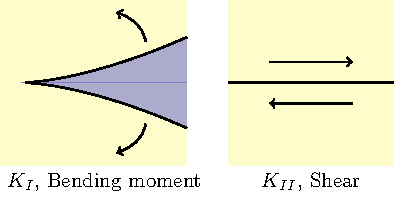
\includegraphics{NumFig3.pdf}
\end{figure}

\textbf{Goal:} 
Find $\lambda$ such that $K_I(\lambda)=0$, ``Zero toughness solution''.
Given this we then want to investigate the behaviour for small $K_I\approx 0$.
To do this, take some given value of $\lambda$ and then solve equations
\ref{eq1}, \ref{eq2}.
\subsection*{Discretization of problem}
The method chosen to discretize the problem is to take a vector 
$(x_1, \dots , x_n)$ of $n$ points at which we measure $g', h'$ and have a 
vector $(z_1, \dots ,z_{n-1})$ of $n-1$ intermediate 
points at which $p$ is measured. The spacing chosen is a $\tan^2$ spacing.
\begin{figure}[!ht]\centering
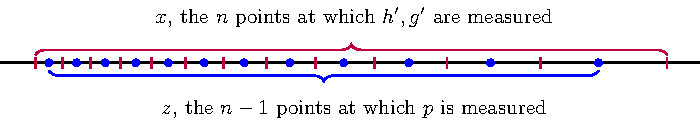
\includegraphics{NumFig2.pdf}
\end{figure}

The ``obvious'' way to interpolate $h'$ in between the $x_i$'s is 
simple linear interpolation. But both $h',g'$ become singular near 0.
However, we expect a $x^{-1/2}$ singularity, which allows us to ``remove''
said singularity. 
The interpolation used is
\[ g'(x) = \left\{ \begin{array}{cc} \frac{1}{\sqrt{x}}(a_ix+b_i) &
i <t \\ a_ix+b_i & i \geq t \end{array} \right. \]
for $x$ in the spline $x \in [x_i,x_{i+1}]$. Choose $1 < t < n$, typically
$t=n/2$. Similarly
\[ h'(x) = \left\{ \begin{array}{cc} \frac{1}{\sqrt{x}}(c_ix+d_i) &
i <t \\ c_ix+d_i & i \geq t \end{array} \right. \]
With the same $t$ used. We will interpolate beyond $x_n$ via 
$g'(x) = a_n x + b_n$, for $x>x_n$, and similar for $h'$.

The values of $g',h'$ are stored via 
\[ \bs{\theta} = \left( \begin{array}{c} a_1x_1+b_1 \\ \vdots 
\\ a_n x_n+b_n \\[4pt] c_1x_1+d_1 \\ \vdots \\ c_n x_n + d_n \end{array} 
\right) \]
Once one has $\bs{\theta}$, it is trivial to recover, say $g'(x_i)$, since
either $g'(x_i) = \bs{\theta}_i$ or $g'(x_i) = \bs{\theta}_i/\sqrt{x_i}$.
Similarly, given $g'(x_i)$; $\bs{\theta}_i$ can be calculated.

\subsection*{Recovering the a$_{i}$'s}
Suppose we know $\bs{\theta}$, (and always assume we know the $x_i$).
Can we recover $a_i, b_i, c_i, d_i$? 
The answer is yes, once we add in the boundary conditions at $\infty$.
Further we have that 
\[ \bs{\gamma} = \left( \begin{array}{c} a_1 \\ \vdots 
\\ a_n \\[3pt] b_1 \\ \vdots \\ b_n \\[3pt] c_1 \\ \vdots \\ c_n 
\\[3pt] d_1 \\ \vdots \\ d_n  \end{array} \right)
= T \bs{\theta} \]
Where T is a $4n \times n$ interpolation matrix. A quick check reveals
we have $4n$ unknowns, in $\bs{\gamma}$. Knowing $\theta$ provides $2n$
equations. Demanding continuity of the interpolated $g',h'$ provides
another $2(n-1)$ equations, (match at $x_2, \dots, x_n$). Finally boundary
conditions on the spline at $\infty$ provide another 2 equations.

The continuity conditions are 
\begin{align*}
a_1 x_2 + b_1 &= a_2 x_2 + b_2 \\
& \;\; \vdots \\
a_{t-2} x_{t-1} + b_{t-2} &= a_{t-1} x_{t-1} + b_{t-1} \\
(a_{t-1} x_{t} + b_{t-1})/\sqrt{x_t} &= a_{t} x_{t} + b_{t} \\
a_{t} x_{t+1} + b_{t} &= a_{t+1} x_{t+1} + b_{t+1} \\
& \;\; \vdots \\
a_{n-1} x_{n} + b_{n-1} &= a_{n} x_{n} + b_{n} \\
\end{align*}
and similar for $c,d$. This means that with the exceptions of
$i=t-1,n$, have that 
\[ \frac{\theta_{i+1}-\theta_i}{x_{i+1}-x_i} = a_i \]
\[ \frac{\theta_{i}\,x_{i+1}-\theta_{i+1}x_i}{x_{i+1}-x_i} = b_i \]
Same idea with $x_{t-1}$, just have to be a little careful about
the switch in the continuity condition,
\[ \frac{\sqrt{x_t}\theta_{t}-\theta_{t-1}}{x_t-x_{t-1}} = a_{t-1} \]
\[ \frac{\theta_{t-1}\,x_t-\theta_t x_{t-1}\sqrt{x_t}}
{x_t-x_{t-1}} = b_{t-1} \]

So we are almost done, just missing 4 rows in our matrix. Have the
$n^{th}$ row as all zeros, i.e. $a_n=0$ due to boundary conditions,
and so trivially the $2n^{th}$ row is 0 except $T_{2n,n} = 1 $
Now, B.C. for $h'$ implies $h''(x_n) \approx h''(x_{n-1})$ i.e.
$c_n=c_{n-1}$ and thus from continuity $d_n=d_{n-1}$. This completes
our interpolation matrix $T$. We still have some extra boundary
conditions to impose, which we will do later. Naively, these
are $g'(x_n) = b_n = 1/2$, $c_n=1$. These are approximately true, but
we need to do a bit better. (I will add this into the explanation
once I understand it$\dots$)  
\\
\subsubsection*{Analytic expressions}
Now that we have made the piecewise analytic approximation\footnote{
I think I have made up some terminology here, piecewise linear isn't
quite right due to the $x^{-1/2}$ parts, and ``sometimes piecewise linear
sometimes piecewise $x^{-1/2}\times$(linear function)'' is not ideal 
either} we can avoid making any more approximations. Recall
$K_{ij}$ has an analytic expression (even better, it's a rational function). 
If we take $h',g'$ to be piecewise
analytic, then the integrand becomes an analytic expression that can
be exactly integrated. For example,

\begin{align*} 
p(z) &= \int_0^{\infty} K_{11}(x-z) g'(x) + K_{12}(x-z) h'(x) \; dx \\
&= \sum_{i=1}^{t-1}\int_0^{\infty} K_{11}(x-z)(a_i x+ b_i)/\sqrt x 
 + K_{12}(x-z) (c_ix+d_i)/\sqrt x \; dx \\
&+ \sum_{i=t}^{n}\int_0^{\infty} K_{11}(x-z)(a_i x+ b_i) 
 + K_{12}(x-z) (c_ix+d_i) \; dx
\end{align*}
The right hand side of this equation may look ghastly, (and we haven't
even expanded the $K_{ij}$'s yet $\dots$) but it is an analytic expression
in $z$. Further, we can do the integration before knowing any of the
values of $a,b,c,d$. It is also clear that $p(z)$ is linear in $a,b,c,d$.
Therefore, once we know the spacing of the $z_i$'s we see that 
\[ \left( \begin{array}{c} p(z_1) \\ \vdots \\ p(z_{n-1}) \\[4pt] 0 \\ \vdots \\
0 \end{array} \right) =
\left( \begin{array}{ccc} B_{1,1} & \cdots & B_{1 , 2n} \\
\vdots & \ddots & \vdots \\ B_{2(n-1),1} & \cdots & B_{2(n-1) , 2n} 
\end{array}
\right) \bs{\gamma} = BT\bs{\theta} \]
Where the matrix $B$ depends on the choice of spacings ($x, z$), but does
not depend on $\bs{\gamma}$.

We can go further and incorporate the boundary conditions into this equation. 
The discretized versions of the boundary conditions, become
$g'(x_n)=1/2$ and $\displaystyle \frac{h'(x_n)-h'(x_{n-1})}{x_n-x_{n-1}} = 1$.
\footnote{Again, we need to do a bit better than this. For now, this 
illustrates the point.}
These conditions are linear in terms of $g',h'$, and so by adding another two 
rows onto the matrix $BT$, get that
\[ \left( \begin{array}{c} p(z_1) \\ \vdots \\ p(z_{n-1}) \\[4pt] 0 \\ \vdots \\
0 \\ g'(\infty) \\ h''(\infty) \end{array} \right) =
\left( \begin{array}{ccc} A_{1,1} & \cdots & A_{1 , 2n} \\
\vdots & \ddots & \vdots \\ A_{2n,1} & \cdots & A_{2n , 2n} 
\end{array}
\right) \bs{\theta}\]
Where $g'(\infty), h''(\infty)$ are the (constant) boundary conditions. 
\\

Now we use the second equation for $p$, namely $p=\int_z^{\infty} 
\lambda/h^2 dx$. We can integrate our piecewise analytic expression
for $h'$ to recover $h$, imposing both $h(x_1)=0$ as well as continuity at the
$x_i$ for $i=2,\dots n$. The result is 
\[ h(x) = \left\{ \begin{array}{cc} \sqrt{x}(w_ix+e_i)+r_i &
i <t \\ w_ix^2+e_ix + r_i & i \geq t \end{array} \right. \]
for some constants $w,e,r$. These constants are related to $\bs{\gamma}$,
and so $\bs{\theta}$, linearly. Given this piecewise analytic expression
for $h$, we can find an analytic expression for $p(z)$. Since we know the
spacings, we have
\[ f(\bs{\theta}) = \left( \begin{array}{c} p(z_1) \\ \vdots \\ p(z_{n-1}) 
\\[4pt] 0 \\ \vdots \\ 0 \\ g'(\infty) \\ h''(\infty) \end{array} \right) =
 A  \bs{\theta} \]
Where we now just need to solve for $\bs{\theta}$.

\subsection*{Newton's method}
Suppose $\bs{\theta}$ is iterate 1. To get the next iterate you need to solve 
(to first order)
\[ f(\bs{\theta}+\delta\bs{\theta}) = A(\bs{\theta}+\delta \bs{\theta})\]
\[ f(\bs{\theta}) + (Df|_{\bs{\theta}})(\delta\bs{\theta}) = A\bs{\theta}+
A\delta \bs{\theta}\]
Where $Df|_{\bs{\theta}}$ is a matrix of partial derivatives. Therefore, get to 
first order that 
\[ \delta \bs{\theta} =  (A-Df|_{\bs{\theta}})^{-1}(f(\bs{\theta}) - A\bs{\theta}) \]

Ingredients:
\begin{itemize}
\item Matrix $A$ itself (of which the $2(n-1)\times2n$ part is the integral
      kernel)
\item The function $f(\bs{\theta})$. I.e. given $\bs{\theta}$ you need to calculate
      $\int_z^{\infty}\lambda/h^2 dx$ (Key functions ``hprime\_to\_h'' and
      ``hprime\_to\_p'').
\item Need to calculate $Df$ which involves calculating $\displaystyle \frac
      {\partial} {\partial \bs{\theta}} \int_z^{\infty} \frac{\lambda}{h(x)^2}dx$

\end{itemize}
So we have worked out numerically $K(\lambda)$, now we want to solve 
$K(\lambda_0)=0$ for $\lambda_0$. We do a ``march''. Sublety in that $K<0$ is 
unphysical, so a guess of $\lambda>\lambda_0$ where $K(\lambda_0)=0$ does
not make any physical sense (\& will get bad numerical results). To get 
around this difficulty, take the next iterate of $\lambda$ as smaller than
predicted.
\begin{figure}[!ht]\centering
\caption{March to find $\lambda_0$}
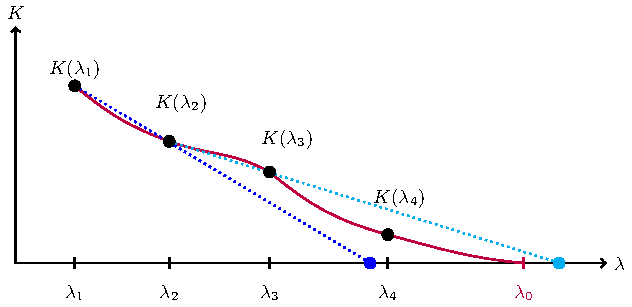
\includegraphics{NumFig1.pdf}\label{March}
\end{figure}

For example in Figure \ref{March}, the obvious choice for $\lambda_4$
(the light blue circle) is larger than the true value of $\lambda_0$, 
and therefore the naive extrapolation method won't quite work.
\clearpage
\section*{Guide to programs}
Important note: What I have called $\bs{\theta}$ in this document is
(confusingly) called hprime in the code. From now on I will call it
$\bs{h}'$, in bold to try to avoid confusion.
\subsection*{\color{blue} \texttt{K\_of\_c\_march}}
First the program sets up the spacing as $\tan^2$. It also sets the
initial $\bs{h}'= (\underbrace{1,\dots,1}_{g'} \underbrace{x_1+1, \dots,
x_n+1}_{h'})$ \textcolor{orange}{(Not sure why this is a reasonable first
guess, perhaps from the boundary conditions at $\infty$. Seems to have
no problems converging though.)}

Most of the work is then done by \texttt{fixed\_lambda\_M\_iteration}
which then solves for $K_I$ and $\bs{h}'$. 

N.B. $\bs{h}'$ is updated via $\displaystyle \bs{h}_i' = \frac{\bs{h}_{i-1}'
-\bs{h}_{i-2}'}{\lambda_{i-1} - \lambda_{i-2}} \lambda_i + 
\frac{\lambda_{i-1}\bs{h}_{i-2}'-\lambda_{i-1}\bs{h}_{i-1}'}
{\lambda_{i-1} - \lambda_{i-2}} $ which is just linear extrapolation.
In the absence of any better ideas this is the sensible choice.

After iterating for a few values, get near $\lambda_0$. Hear we suspect
that something like $K^3 \sim \lambda-\lambda_0$ near $\lambda=\lambda_0$,
$K=0$. So given two prior guesses, extrapolate via 
$\displaystyle \lambda_i = \frac{K_{i-1}^3\lambda_{i-2} - K_{i-2}^3
\lambda_{i-1}}{K_{i-1}^3-K_{i-2}^3}$ But as noted earlier, must be careful
to not extrapolate further than $\lambda_0$. So an idea is to take $(\lambda_i
+ \lambda_{i-1})/2$ as the next guess, i.e. 
\[\lambda_i = 
\frac{\lambda_{i-1} - \lambda_{i-2}}{K_{i-1}^3-K_{i-2}^3}\frac{K_{i-1}^3}{2}
+ \frac{K_{i-1}^3\lambda_{i-2} - K_{i-2}^3 
\lambda_{i-1}}{K_{i-1}^3-K_{i-2}^3} \]
Then the program just iterates. If it doesn't converge, it simply tries a 
smaller value of $\lambda$.

\subsection*{\color{blue} \texttt{fixed\_lambda\_M\_iteration}}
Takes a value of $\lambda$ and returns the corresponding $K$ value.
Now using the ``scaled'' version, so the values of $P,M$ are implicitly
assumed to be $0,1$ respectively.

\textcolor{red}{Somewhat concerningly, $\bs{h}'$ is assumed to 
already have this spacing, which could potentially cause issues.
If you wanted to change the spacing you would have to do it in
two different places.}

Subroutines then return the kernel matrix \& the interpolate matrix.
The kernel matrix is in lieu of $\displaystyle \left( \begin{array}{c}
p \\ 0 \end{array} \right) = \int \underline{\underline{K}} \left(
\begin{array}{c} g' \\ h' \end{array} \right) $.
The interpolate matrix actually only appears here to add in boundary
conditions to the matrix $A$.

The matrix $A$ is set up, which is part kernel, part interpolate matrix,
same matrix as described earlier.

The rcond statement is testing how conditioned the matrix $A$ is, or how 
ameniable it is to being numerically inverted. There does not seem to be
a huge amount of point in adding this step in.

Then the iteration loop begins. Follows Newton's method for the equation
$f(\bs{h}') = A \bs{h}'$ and iterates via $\displaystyle \bs{h}'_{new} =
\bs{h}'_{old} + (A-Df|_{\bs{h}_{old}'})^{-1}(f(\bs{h}_{old}') - A\bs{h}_{old}')$
Where we already know $A$. $f, Df$ are provided via \texttt{hprime\_to\_p}
and $f, Df$ are called $p, dp$ respectively in the program.

\subsection*{\color{blue} \texttt{pprime\_to\_p}}
This function is given $h,x,z$ ($h$ in the form of the h\_coeff vector)
and returns 
$\displaystyle \frac{1}{\lambda} \left( \begin{array}{c} p(z_1) \\ \vdots \\
p(z_{n-1}) \end{array} \right) $ via the equation $\displaystyle p =-\lambda
 \int_z^{\infty} \frac{1}{h^2} dx$
\\

Again, once one has made the approximation of $h$ as piecewise analytic, can 
actually work out the exact integrals. So all this function really has to do
is to evaluate some known functions, plugging in the values of h\_coeff.


\subsection*{\color{blue} \texttt{pressure\_map\_derivative}}
This function calculates $Df$ or $\frac{\partial}{\partial \bs{\theta}} f$.
Most of $f$ is either zeros, or the boundary conditions which we assume to
be constant. (actually, our more refined guess of the boundary conditions makes
them non-constant, but \texttt{bending\_p\_adjust} will do these corrections.

The easiest way to think of $p$ is as a function of the coefficients of $h$,
i.e. the $w,e,r$. So $p(z) = p(z;w,e,r)$, and actually we can find analytic
expressions for things like $\frac{\partial}{\partial e_i} p$. Now there is 
a linear relationship between $(w,e,r)$ and $\bs{\theta}$, say 
$(w,e,r) = H \bs{\theta}$ where $H$ is the h\_coeff matrix, provided by
\texttt{h\_coefficient\_matrix.m}

We use this, together with the chain rule, to find an expression for $Df$.

\subsection*{\color{blue} \texttt{hprime\_to\_p}}
finds $p$ and $dp$ given $\bs{h}'$
The pressure is found via \texttt{pprime\_to\_p}. dp is found via
\texttt{pressure\_map\_derivative}.

Then \texttt{bending\_p\_adjust} corrects the shoddy boundary conditions
in both $p$ and $dp$.

\subsection*{\color{blue} \texttt{hprime\_to\_h}}
This function takes $h'$ and returns $H$ the coefficient matrix for $h$.
Starting point, suppose we know the $c,d$ coefficients for $h'$.
Then have that 
$$ h'(x) = \left\{ \begin{array}{cc} \frac{1}{\sqrt{x}}(c_ix+d_i) &
i <t \\ c_ix+d_i & i \geq t \end{array} \right. \;\; x \in [x_i,x_{i+1}] $$
Then integrating gives that 
$$ h'(x) = \left\{ \begin{array}{cc} w_ix^{3/2}+e_ix^{1/2}+r_i &
i <t \\ w_ix^2+e_i x + r_i & i \geq t \end{array} \right. \;\; x 
\in [x_i,x_{i+1}] $$
where
$$ w_i = \left\{ \begin{array}{cc} \frac{2}{3} c_i &
i <t \\[4pt] \frac{1}{2}c_i & i \geq t \end{array} \right.  $$

$$ e_i = \left\{ \begin{array}{cc} 2d_i &
i <t \\[4pt] d_i & i \geq t \end{array} \right.  $$

We recover the $r_i$'s through imposing continuity and $c_1=0$. Get
that

$$ r_i = \left\{ \begin{array}{cc} r_i + \frac{2}{3}(c_i-c_{i+1})x^{3/2}_{i+1}
+2(d_i-d_{i+1})x^{2/3}_{i+1} & i <t \\[4pt] 
r_{i+1} + \frac{1}{2}(c_i-c_{i+1})x^2_{i+1} +(d_i-d_{i+1})x_{i+1} & 
i \geq t \end{array} \right.  $$
Which looks complicated, but can see that $r$ is related to $c,d$ linearly. 

So all this function does is return a matrix $H$.
Important note: The coefficients of $h$ are stored
$(w_1,e_1,r_1, \dots, w_n,e_n,r_n)$, rather than what you might expect, 
$(w_1,\dots, w_n, e_1, \dots, e_n, r_1, \dots, r_n)$. (For reasons unknown)

\subsection*{\color{blue} \texttt{pressure\_shear\_matrix}}
This function finds the matrix which replaces the elastic integral.
Recall that once we make the piecewise analytic approximation, we can 
do all the integrals exactly. The resulting functions are stored in this 
program. 

\end{document}
